% =============================================================================
% Multimodal deepfake detection: IEEE conference-format paper (deliverables v2).
% Class: IEEEtran_nodash, [conference] option (two-column, 10 pt). Overleaf
% compatible: relative paths only, packages shipped with TeX Live and MiKTeX.
% Build: latexmk -g -pdf -interaction=nonstopmode main.tex
%
% Rules in force (CLAUDE.md, deliverables_v2/SPEC.md):
%   - Every number is copied from deliverables_v2/CONTENT_MAP.md, with the same
%     decimals and the same label (exploratory, sealed, post hoc, engineering).
%     Experiment and decision IDs appear only in LaTeX comments.
%   - Only keys of refs.bib with READ or PARTIAL status in docs/RESEARCH.md.
%   - No em-dashes or en-dashes. No unsupported superlatives or speed claims.
% =============================================================================
\newif\ifcollegestyle
\collegestyletrue
%\collegestylefalse

\ifcollegestyle
  \documentclass[conference,a4paper]{IEEEtran_nodash}
\else
  \documentclass[conference]{IEEEtran_nodash}
\fi

\usepackage[T1]{fontenc}
\usepackage[utf8]{inputenc}
\usepackage{amsmath,amssymb}
\usepackage{booktabs}
\usepackage{array}
\newcolumntype{L}[1]{>{\raggedright\arraybackslash}p{#1}}
\usepackage{graphicx}
% project rule: no dashes; the cite package would join ranges with an en dash
\makeatletter\def\citedash {\hbox{-}}\makeatother
\usepackage{cite}
\usepackage[hidelinks,hypertexnames=false,pdftitle={Multimodal Deepfake Detection for Images, Video and Audio},pdfauthor={Shivansh Gupta, Vaibhav Shiroorkar, Adithya Jithesh}]{hyperref}

\graphicspath{{figures/}}

% Title: ONE definition, used by the cover, the certificate and the paper title block.
\newcommand{\papertitle}{Multimodal Deepfake Detection for Images, Video and Audio}
% Hook that college-style.tex redefines; in plain mode it does nothing.
\newcommand{\collegetitlecolour}[1]{#1}
\ifcollegestyle
  % =====================================================================
% college-style.tex : the K. J. Somaiya School of Engineering look, layered on IEEEtran.
% Loaded by main.tex ONLY when \collegestyletrue. With \collegestylefalse none of this runs and
% main.tex produces the plain IEEEtran conference paper. The layout follows the college-branded
% reference paper of another project (layout and style only; no text of that project is used).
%
% What this file changes (and nothing else):
%   1. Colours: maroon #B7202F and dark brown #312016, sampled from the college reference report.
%   2. A thin maroon border (1.2 pt, 1 cm inside the page edge) on every page, cover included.
%   3. A footer (maroon rule, bold department/semester/batch text, bold "Page n") on every page
%      except the cover, drawn at fixed positions independent of the IEEEtran margins.
%   4. Paper title and level-1 headings in maroon, level-2 and level-3 headings in dark brown
%      (the IEEEtran heading definitions are copied unchanged except for the colour).
%   5. Front matter in single-column Times 12 pt with the reference margins: cover, certificate,
%      declaration, acknowledgements, contents, list of figures, list of tables, abbreviations,
%      roman page numbers from the certificate. The IEEEtran two-column body restarts at page 1.
% Only packages shipped with TeX Live are used: eso-pic, xcolor, geometry, graphicx, array.
% =====================================================================
\makeatletter
\usepackage{eso-pic}
\usepackage{xcolor}
\usepackage{array}
% geometry in "pass" mode does not touch the IEEEtran layout; it is used only to give the front
% matter the reference margins and to restore the IEEEtran layout for the paper.
\usepackage[pass]{geometry}

% ---------------------------------------------------------------- colours
\definecolor{collegemaroon}{HTML}{B7202F}
\definecolor{collegebrown}{HTML}{312016}

% ---------------------------------------------------------------- fonts
\newcommand{\collegefont}{\fontfamily{ptm}\selectfont}
\newcommand{\collegefrontbody}{\collegefont\fontsize{12}{14.5}\selectfont}
\newcommand{\collegesize}[1]{%  sizes used in the reference (pt)
  \ifcase#1\or\fontsize{12}{14.5}\or\fontsize{14.4}{17.5}\or\fontsize{17.28}{21}\or\fontsize{24.88}{30}\fi\selectfont}

% ---------------------------------------------------------------- footer text
\newcommand{\collegefootertext}{Department of Electronics and Computer Engineering\hspace{2em}Semester VII\hspace{2em}2026-27 Batch}

% ---------------------------------------------------------------- border and footer (every page)
\newif\ifcollegefooter
\collegefooterfalse          % off for the cover; switched on after the cover is shipped out
\newcommand{\cs@pt}[1]{\strip@pt\dimexpr#1\relax}
\AddToShipoutPictureBG{%
  \begingroup
  \setlength{\unitlength}{1pt}%
  \color{collegemaroon}%
  % border: four 1.2 pt rules, 1 cm inside each page edge
  \put(\cs@pt{1cm},\cs@pt{1cm}){\rule{\dimexpr\paperwidth-2cm\relax}{1.2pt}}%
  \put(\cs@pt{1cm},\cs@pt{\paperheight-1cm-1.2pt}){\rule{\dimexpr\paperwidth-2cm\relax}{1.2pt}}%
  \put(\cs@pt{1cm},\cs@pt{1cm}){\rule{1.2pt}{\dimexpr\paperheight-2cm\relax}}%
  \put(\cs@pt{\paperwidth-1cm-1.2pt},\cs@pt{1cm}){\rule{1.2pt}{\dimexpr\paperheight-2cm\relax}}%
  % footer: 1 pt maroon rule 1.93 cm above the bottom edge, text baseline 1.5 cm, spanning
  % 2.54 cm from the left to 2 cm from the right edge (the reference text width)
  \ifcollegefooter
    \put(\cs@pt{2.54cm},\cs@pt{1.93cm}){\rule{\dimexpr\paperwidth-4.54cm\relax}{1pt}}%
    \put(\cs@pt{2.54cm},\cs@pt{1.5cm}){\makebox[\dimexpr\paperwidth-4.54cm\relax][l]{%
      \color{black}\normalfont\collegefont\fontsize{10}{12}\selectfont\bfseries\upshape
      \collegefootertext\hfill Page \thepage}}%
  \fi
  \endgroup}

% ---------------------------------------------------------------- heading colours (IEEEtran definitions, colour added)
\def\section{\@startsection{section}{1}{\z@}{1.5ex plus 1.5ex minus 0.5ex}%
{0.7ex plus 1ex minus 0ex}{\normalfont\normalsize\centering\scshape\color{collegemaroon}}}
\def\subsection{\@startsection{subsection}{2}{\z@}{1.5ex plus 1.5ex minus 0.5ex}%
{0.7ex plus .5ex minus 0ex}{\normalfont\normalsize\itshape\color{collegebrown}}}
\def\subsubsection{\@startsection{subsubsection}{3}{\parindent}{0ex plus 0.1ex minus 0.1ex}%
{0ex}{\normalfont\normalsize\itshape\color{collegebrown}}}
\renewcommand{\collegetitlecolour}[1]{\textcolor{collegemaroon}{#1}}

% ---------------------------------------------------------------- table of contents
\setcounter{tocdepth}{2}
\renewcommand\contentsname{Contents}
% Top-level entries bold without dot leaders, like the reference; subsections keep dotted lines.
\newcommand*\l@frontmatter[2]{\addpenalty{\@secpenalty}\addvspace{0.35em}%
  \begingroup\parindent\z@\rightskip\@pnumwidth\parfillskip-\@pnumwidth
  \leavevmode\bfseries #1\nobreak\hfil\nobreak\hb@xt@\@pnumwidth{\hss #2}\par\endgroup}
\renewcommand*\l@section[2]{\addpenalty{\@secpenalty}\addvspace{0.45em}%
  \begingroup\parindent\z@\rightskip\@pnumwidth\parfillskip-\@pnumwidth
  \leavevmode\bfseries\@tempdima 2.75em #1\nobreak\hfil\nobreak
  \hb@xt@\@pnumwidth{\hss #2}\par\endgroup}
\renewcommand\tableofcontents{\collegefrontheading{\contentsname}{\small\@starttoc{toc}}}
\renewcommand\listoffigures{\collegefrontheading{\listfigurename}\@starttoc{lof}}
\renewcommand\listoftables{\collegefrontheading{\listtablename}\@starttoc{lot}}
% Roomier number column and wider page-number column for the long entries.
\renewcommand*\l@subsection{\@dottedtocline{2}{1.5em}{3.2em}}
\renewcommand*\l@figure{\@dottedtocline{1}{0em}{2.8em}}
\let\l@table\l@figure
\renewcommand*\@pnumwidth{2.2em}

% ---------------------------------------------------------------- front-matter building blocks
\newcommand{\collegefrontheading}[1]{%   left-aligned maroon heading (Acknowledgements, Contents, lists)
  \vspace*{0.6cm}\noindent{\collegefont\collegesize{4}\bfseries\color{collegemaroon}#1\par}\vspace{26pt}}
\newcommand{\collegecentredheading}[1]{% centred maroon heading (Certificate, Declaration)
  \begin{center}\collegefont\collegesize{4}\bfseries\color{collegemaroon}#1\end{center}\vspace{18pt}}
% Reference margins for the front matter only: left 2.54 cm, right 2 cm, no header.
\newcommand{\collegefrontgeometry}{\newgeometry{left=2.54cm,right=2cm,top=1.9cm,bottom=3cm,nohead}}
\newcommand{\collegeinstitutionheader}{%
  \begin{center}\collegefont\bfseries
  {\collegesize{3}\color{collegebrown}Somaiya Vidyavihar University\par}\vspace{14pt}
  {\collegesize{3}K. J. Somaiya School of Engineering\par}
  \end{center}\vspace{26pt}}
\newcommand{\collegesignline}{\rule{5.2cm}{0.4pt}}
\newcommand{\collegefrontpage}[1]{% start a front-matter page and list it in the contents (roman number)
  \clearpage\addcontentsline{toc}{frontmatter}{#1}}

% ---------------------------------------------------------------- the people (identity fields)
\newcommand{\collegestudents}{%
  Shivansh Gupta/16014023052/Vaibhav Shiroorkar/16014024805/Adithya Jithesh/16014024803}
\newcommand{\collegestudentrow}[3]{#1 & #2 & #3}

% ---------------------------------------------------------------- cover (border, no footer)
\newcommand{\collegecover}{%
  \thispagestyle{empty}
  \begingroup\centering\collegefont
  \IfFileExists{figures/somaiya_vidyavihar_logo.jpg}%
    {
\includegraphics[width=7.4cm]{figures/somaiya_vidyavihar_logo.jpg}\par}%
    {\textbf{Somaiya Vidyavihar University}\par}
  \vspace{0.6cm}
  {\collegesize{3}\bfseries\color{collegebrown}Somaiya Vidyavihar University\par}
  \vspace{0.25cm}
  {\collegesize{2}\bfseries K. J. Somaiya School of Engineering\par}
  \vspace{0.15cm}
  {\collegesize{2}\bfseries Department of Electronics and Computer Engineering\par}
  \vspace{0.8cm}
  {\collegesize{4}\bfseries\color{collegemaroon}\papertitle\par}
  \vspace{0.8cm}
  {\collegesize{1}Submitted In Partial Fulfillment of Requirements\par For the Degree Of\par}
  \vspace{0.3cm}
  {\collegesize{3}\bfseries Bachelor of Technology\par}
  \vspace{0.1cm}
  {\collegesize{2}\bfseries (Electronics and Computer Engineering)\par}
  \vspace{0.6cm}
  {\collegesize{1}By\par}
  \vspace{0.2cm}
  {\collegesize{1}%
  \begin{tabular}{@{}l@{\hspace{2.2cm}}l@{}}
    \textbf{\collegesize{2}Shivansh Gupta} & Roll No: 16014023052\\[3pt]
    \textbf{\collegesize{2}Vaibhav Shiroorkar} & Roll No: 16014024805\\[3pt]
    \textbf{\collegesize{2}Adithya Jithesh} & Roll No: 16014024803\\
  \end{tabular}\par}
  \vspace{0.6cm}
  {\collegesize{1}Guide\par}
  \vspace{0.2cm}
  {\collegesize{3}\bfseries Dr. Tejashree Phatak\par}
  {\collegesize{1}Assistant Professor\par}
  \vfill
  {\collegesize{2}\bfseries Somaiya Vidyavihar University\par}
  {\collegesize{1}Vidyavihar, Mumbai - 400 077\par}
  \vspace{0.2cm}
  {\collegesize{2}\bfseries 2026-2027\par}
  \endgroup}

% ---------------------------------------------------------------- certificate
\newcommand{\collegecertificate}{%
  \collegefrontpage{Certificate}
  \begingroup\collegefrontbody
  \collegeinstitutionheader
  \collegecentredheading{Certificate}
  \noindent This is to certify that the project report entitled ``\textbf{\papertitle}''
  submitted by the following students at the end of Semester VII of LY B.\ Tech is a bona fide record for
  partial fulfillment of requirements for the degree of \textbf{Bachelor of Technology (Electronics and
  Computer Engineering)} of Somaiya Vidyavihar University.\par
  \vspace{0.6cm}
  \noindent\begin{tabular}{@{}p{6.6cm}@{}l@{}}
    \textbf{Shivansh Gupta} & (16014023052)\\[3pt]
    \textbf{Vaibhav Shiroorkar} & (16014024805)\\[3pt]
    \textbf{Adithya Jithesh} & (16014024803)\\
  \end{tabular}\par
  \vspace{1.6cm}
  \noindent\begin{tabular}{@{}p{0.5\linewidth}@{}p{0.48\linewidth}@{}}
    \collegesignline & \collegesignline\\[2pt]
    \textbf{Guide} & \textbf{Head of the Department}\\[2pt]
    Dr.\ Tejashree Phatak & Dr.\ Jagannath Nirmal\\[1.5cm]
    \collegesignline & \collegesignline\\[2pt]
    \textbf{Examiner} & \textbf{Director}\\
  \end{tabular}\par
  \vspace{1.2cm}
  \noindent\textbf{Date:}\par\medskip
  \noindent\textbf{Place:} Mumbai-77\par
  \endgroup}

% ---------------------------------------------------------------- declaration (framed signature cells, three students)
\newcommand{\collegesigncell}[2]{%
  \begin{minipage}[t]{0.3\linewidth}\raggedright\vspace{4pt}
  \textbf{Signature of the Student}\par\vspace{1.0cm}
  \rule{\dimexpr\linewidth-0.4cm\relax}{0.4pt}\par\vspace{2pt}
  \textbf{#1}\par
  \textbf{Roll No.} #2\par\vspace{4pt}
  \end{minipage}}
\newcommand{\collegedeclaration}{%
  \collegefrontpage{Declaration}
  \begingroup\collegefrontbody
  \collegeinstitutionheader
  \collegecentredheading{Declaration}
  \noindent We declare that this written report submission represents the work done based on our and/or others'
  ideas with adequately cited and referenced the original source. We also declare that we have adhered to all
  principles of intellectual property, academic honesty and integrity as we have not misinterpreted or fabricated
  or falsified any idea/data/fact/source/original work/matter in our submission.\par
  \medskip
  \noindent We understand that any violation of the above will be cause for disciplinary action by the college and
  may evoke the penal action from the sources which have not been properly cited or from whom proper permission is
  not sought.\par
  \vspace{1cm}
  \noindent\fbox{\collegesigncell{Shivansh Gupta}{16014023052}}\hfill
  \fbox{\collegesigncell{Vaibhav Shiroorkar}{16014024805}}\hfill
  \fbox{\collegesigncell{Adithya Jithesh}{16014024803}}\par
  \vspace{0.8cm}
  \noindent\textbf{Date:}\par\medskip
  \noindent\textbf{Place:} Mumbai-77\par
  \endgroup}

% ---------------------------------------------------------------- acknowledgements
\newcommand{\collegeacknowledgements}{%
  \collegefrontpage{Acknowledgements}
  \begingroup\collegefrontbody
  \collegefrontheading{Acknowledgements}
  \noindent We would like to express our sincere gratitude to our project guide, Dr.\ Tejashree Phatak, Assistant
  Professor, Department of Electronics and Computer Engineering, K.\ J.\ Somaiya School of Engineering, for her
  guidance, advice and encouragement throughout this project.\par
  \medskip
  \noindent We thank Dr.\ Jagannath Nirmal, Head of the Department of Electronics and Computer Engineering, for
  the facilities that made the work possible, and the faculty and staff of the Department of Electronics and
  Computer Engineering and of K.\ J.\ Somaiya School of Engineering, Somaiya Vidyavihar University, for their
  support.\par
  \medskip
  \noindent We acknowledge the authors of the datasets used in this work, FaceForensics++, Celeb-DF, Celeb-DF++,
  DeepFakeDetection, ASVspoof 2019, In-the-Wild, LAV-DF, FakeAVCeleb, DeepAction, DF26, Community Forensics and
  the ForenSynths generated-image sets, who made them
  available for research, and the developers of the open-source software on which the project is built, among
  them PyTorch, timm, Hugging Face Transformers, OpenCV and Flask.\par
  \medskip
  \noindent Finally we thank our families and friends for their patience and support.\par
  \endgroup}

% ---------------------------------------------------------------- abbreviations (two-column Term / Expansion)
\newcommand{\collegeabbreviations}{%
  \collegefrontpage{Abbreviations}
  \begingroup\collegefrontbody
  \collegefrontheading{Abbreviations}
  \noindent\begin{tabular}{@{}>{\raggedright\arraybackslash}p{2.6cm}%
                          >{\raggedright\arraybackslash}p{\dimexpr\linewidth-2.6cm-2\tabcolsep\relax}@{}}
  \textbf{Term} & \textbf{Expansion}\\[4pt]
  AUC & Area Under the ROC Curve\\
  C2PA & Coalition for Content Provenance and Authenticity\\
  CLIP & Contrastive Language-Image Pre-training\\
  CNN & Convolutional Neural Network\\
  DFD & DeepFakeDetection (dataset)\\
  DFDC & DeepFake Detection Challenge\\
  ECE & Expected Calibration Error\\
  EER & Equal Error Rate\\
  FNR, FPR & False-Negative Rate, False-Positive Rate\\
  GAN & Generative Adversarial Network\\
  GPU & Graphics Processing Unit\\
  JPEG & Joint Photographic Experts Group\\
  LA & Logical Access (ASVspoof 2019)\\
  NLL & Negative Log-Likelihood\\
  ROC & Receiver Operating Characteristic\\
  TPR & True-Positive Rate\\
  rPPG & remote Photoplethysmography\\
  SNR & Signal-to-Noise Ratio\\
  SSL & Self-Supervised Learning\\
  T-A, T-I, T-V & speech task, generated-image task, face-video task\\
  ViT & Vision Transformer\\
  \end{tabular}\par
  \bigskip
  \noindent Dataset and model names (for example FaceForensics++, Celeb-DF, LAV-DF, DINOv2, WavLM) are proper
  names and are not expanded.\par
  \endgroup}

% ---------------------------------------------------------------- the whole front matter, in order
\newcommand{\collegefrontmatter}{%
  \collegefrontgeometry
  \onecolumn
  \pagestyle{empty}%
  \collegecover                      % unnumbered; border, no footer
  \clearpage                        % the cover is shipped out before the footer is switched on
  \global\collegefootertrue
  \pagenumbering{roman}%             % i, ii, ... from the certificate
  \collegecertificate
  \collegedeclaration
  \collegeacknowledgements
  \clearpage{\collegefrontbody\tableofcontents}%
  \collegefrontpage{\listfigurename}{\collegefrontbody\listoffigures}%
  \collegefrontpage{\listtablename}{\collegefrontbody\listoftables}%
  \collegeabbreviations
}
\newcommand{\collegestartpaper}{%   IEEEtran layout back; arabic page numbers from the first page of the paper
  \clearpage\restoregeometry\pagenumbering{arabic}\setcounter{page}{1}\pagestyle{empty}}

\makeatother

\fi

\newcommand{\sigmoid}{\sigma}
\newcommand{\spl}[1]{\texttt{#1}}
\newcommand{\ci}[2]{[#1,\,#2]}

\hyphenation{Cele-b-DF Face-Foren-sics wav-LM}

\begin{document}

\title{\collegetitlecolour{\papertitle}}

\author{%
\IEEEauthorblockN{\begin{tabular}{@{}*{3}{>{\centering\arraybackslash}p{0.3\textwidth}}@{}}
Shivansh Gupta & Vaibhav Shiroorkar & Adithya Jithesh
\end{tabular}}
\IEEEauthorblockA{Department of Electronics and Computer Engineering\\
K. J. Somaiya School of Engineering, Somaiya Vidyavihar University\\
Vidyavihar, Mumbai - 400 077}
\IEEEauthorblockN{Dr. Tejashree Phatak (Guide)}
\IEEEauthorblockA{Assistant Professor}}

\ifcollegestyle
  \collegefrontmatter   % cover, certificate, declaration, acknowledgements, contents, lists, abbreviations
  \collegestartpaper    % clear page, restore the IEEEtran layout, arabic page numbers from 1
\fi

\maketitle

%%%%%%%%%%%%%%%%%%%%%%%%%%%%%%%%%%%%%%%%%%%%%%%%%%%%%%%%%%%%
\begin{abstract}
Published deepfake detectors are compared under different protocols. We build a detector for images,
videos and the speech in videos as a documented path: one frozen pretrained
encoder with a linear head per task, then iterations whose hypotheses and pass
lines were written before each run. Splits are group-disjoint, tuning uses a
development slice, sealed test sets are read once per frozen iteration, and
three paired group-bootstrap tests were declared before that read. On the sealed
Celeb-DF family (7\,650 videos, 344 groups: 44 identities and 300 single YouTube
videos) the final video system, a fine-tuned SigLIP encoder, reaches an AUC of
0.8218 against 0.6238 for the working version (+0.1980 [+0.1688, +0.2242]). It is
non-inferior (margin 0.0100) to an Xception baseline re-run at 224 px; the
declared 95\,\% superiority rule was met (+0.0176 [+0.0025, +0.0327]) but does
not survive Bonferroni correction over the three tests. On sealed In-the-Wild
speech (42 speakers) the final system reaches 0.9148 against 0.7516 (+0.1633
[+0.1177, +0.2266]); part of this gain removes a silence and level shortcut, so
it is not all better detection of synthesis. The ProGAN-trained image probe
misses 0.7395 of the images of 21 recent generators. On LAV-DF a fused
audio-visual score looked near perfect, but its visual part is at chance within
the produced videos (0.5032), so no audio-visual detection is claimed. On
FakeAVCeleb the pre-stated criteria were met, but codec metadata alone separates
real from fake video (0.9985), so they are not evidence of detection quality;
thresholds do not transfer.
\end{abstract}

\begin{IEEEkeywords}
deepfake detection, multimodal, evaluation protocol, frozen encoders, group
bootstrap, sealed test
\end{IEEEkeywords}

%%%%%%%%%%%%%%%%%%%%%%%%%%%%%%%%%%%%%%%%%%%%%%%%%%%%%%%%%%%%
\section{Introduction}\label{sec:intro}

Face swaps, talking-face synthesis, generated images and cloned voices can be
produced with consumer hardware and public software~\cite{dolhansky2020dfdc}. A
useful checker has to accept an image, a video or the audio of a video, and say
how far its output can be trusted. Published numbers come from different
protocols: in one benchmark in which every detector was trained on
FaceForensics++ (c23), a plain Xception network reached an average AUC of 0.9450
on the within-domain test sets and 0.7718 on the cross-domain
ones~\cite{yan2023deepfakebench}. % R-017, their protocol
A single in-dataset number therefore says little about new material, and the
headline of this work is always a dataset never used in training.

Our goal was a final-year engineering project with two parts of equal weight: a
working local system and a record of how it was built. We built the simplest
end-to-end detector first, read its diagnostics, and changed one thing at a time,
each change starting from a hypothesis, a success line and a failure line written
before the run. Failed changes stay in the record.

\paragraph*{Contributions}
(1) A written evaluation protocol: group-disjoint splits, a development slice
separate from sealed test sets, a guarded and logged single reading of each
frozen iteration, paired group-bootstrap statistics, and three confirmatory tests
declared before any sealed read (Section~\ref{sec:protocol}). (2) An encoder
selection rule that prefers the cheapest candidate when the evidence does not
separate it from the leader, and a measured path of seven experimental iterations
with the reason each change was kept or dropped (Sections~\ref{sec:method} and
\ref{sec:results}). (3) Sealed confirmatory results for face video and speech,
with the negative results that limit them.

\paragraph*{What is not claimed}
No audio-visual detection or fused verdict, no pulse-based detection, no
generated-video detection, no detection of images from modern generators, no
temporal localisation and no Gemini capability. Published numbers are given as
context; the only directly comparable row is the re-run Xception baseline.

%%%%%%%%%%%%%%%%%%%%%%%%%%%%%%%%%%%%%%%%%%%%%%%%%%%%%%%%%%%%
\section{Related Work}\label{sec:related}

\paragraph*{Face forgery and generated images}
FaceForensics++ reports that detectors lose accuracy as compression
increases~\cite{rossler2019faceforensics}; Celeb-DF was the hardest of the
datasets its authors compared~\cite{li2020celebdf}, and Celeb-DF++ adds 21 newer
methods~\cite{li2025celebdfpp}. DeepfakeBench finds plain backbones close to
elaborate methods under shared settings~\cite{yan2023deepfakebench}, and detectors
trained on FaceForensics++ can learn its identities~\cite{dong2023implicit}, which
is why splits must keep identities apart. A linear probe on frozen features of a
vision-language model generalised across image generators in its authors'
tests~\cite{ojha2024universal}, and a linear support vector machine on CLIP
features trained on few examples of one generator was evaluated on many
generators~\cite{cozzolino2024raising}. The protocol of training on ProGAN images
comes from a study of CNN-generated images~\cite{wang2020cnnspot}. DF26 benchmarks
detectors on recent open and commercial video generators~\cite{shykula2026df26}.

\paragraph*{Speech, audio-visual and physiological cues}
ASVspoof~2019 is the standard database of synthesised and converted speech with
unseen attacks in its evaluation set~\cite{wang2020asvspoof}; AASIST applies graph
attention to the raw waveform~\cite{jung2021aasist}; models trained on it degrade
strongly on In-the-Wild recordings~\cite{muller2022inthewild}, and frozen
self-supervised encoders with a simple back end transfer
well~\cite{pascu2024generalisable}. FakeAVCeleb provides visual and cloned-voice
manipulations~\cite{khalid2022fakeavceleb}; LAV-DF regenerates only the edited
segments~\cite{cai2022lavdf}. Pulse signals were proposed as
evidence~\cite{ciftci2020fakecatcher}, but high-quality fakes can carry a
pulse~\cite{seibold2025heart} and an independent reproduction reported a much
lower AUC~\cite{harraq2026physio}.

\paragraph*{Encoders and calibration}
Our candidates are generic pretrained encoders: supervised
CNNs~\cite{chollet2017xception,tan2019efficientnet}, self-supervised vision
transformers~\cite{oquab2024dinov2}, image-text
encoders~\cite{radford2021clip,zhai2023siglip}, self-supervised speech
encoders~\cite{baevski2020wav2vec2,hsu2021hubert,chen2022wavlm} and a weakly
supervised recogniser~\cite{radford2023whisper}. Transfer accuracy depends on the
source model in ways that need measuring~\cite{kornblith2019better}. Temperature
scaling, one parameter fitted on validation data, is an effective calibration
correction on the tasks its authors studied~\cite{guo2017calibration}.

\paragraph*{Gap}
Published numbers rarely share data, split and metric, and few studies keep a
development slice apart from a test set that is read once. We ask a narrower
question: on a protocol fixed in advance, how far does a simple multimodal system
get, and what does each change buy?

%%%%%%%%%%%%%%%%%%%%%%%%%%%%%%%%%%%%%%%%%%%%%%%%%%%%%%%%%%%%
\section{System and Method}\label{sec:method}

\subsection{Tasks and score semantics}
Let $x$ be an image, a video or an audio clip and $y\in\{0,1\}$ its label
($y=1$: manipulated). There are three tasks: face video (T-V), generated images
(T-I) and speech (T-A). A video with an audio track gets a visual and an audio
result side by side (Fig.~\ref{fig:pipeline}); there is no combining rule and no
temporal localisation. Detector scores are temperature-scaled on each detector's
validation split, which makes them a probability only for content like that
split; on other sources their reliable property is their order, and no output is
the probability that a file is fake. The frozen detectors are served by a local,
eight-module analysis platform that reports one finding per module with its tested
scope and no overall score; its design, wording rules and software tests (713
passed, 2 skipped (opt-in GPU tests), 13 deselected (data-dependent tests)) are in
the technical report.

\begin{figure*}[!t]
\centering
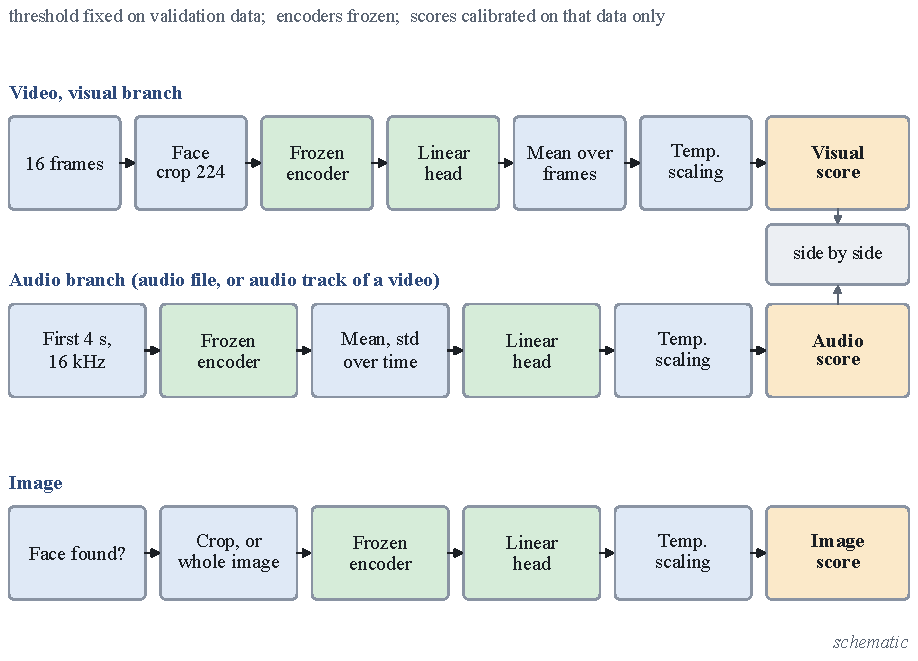
\includegraphics[width=0.8\textwidth]{fig01_pipeline.pdf}
\caption[Three scoring paths]{The three scoring paths of the first version.
Encoders are frozen, heads are linear, each score is temperature-scaled on the
validation split of its task. Visual and audio scores are not fused.}
\label{fig:pipeline}
\end{figure*}

\subsection{Preprocessing, head, calibration and threshold}
One shared package prepares inputs for training, evaluation and inference. A video
gives 16 uniformly spaced frames; the YuNet detector~\cite{wu2023yunet} finds the
largest face, which is enlarged by 1.3, cropped to $224\times224$ and passed
through a JPEG round trip at quality 95; frames without a face are left out. An
image is face-cropped if a face is found and otherwise processed whole by the
encoder's own processor. Audio uses the first 64\,600 samples at 16\,kHz,
repeat-padded if shorter. A hash of this configuration is stored in every
checkpoint and checked at load. For each task one pretrained encoder $\phi$ is
frozen and a linear head $z=\mathbf{w}^{\top}\tilde\phi(x)+b$ is trained on
standardised features with a class-balanced binary cross-entropy, AdamW (learning
rate $10^{-3}$, weight decay $10^{-4}$), early stopping with patience 10 and three
head seeds. For a video with face
frames $F$,
\begin{equation}
s(x)=\sigmoid\!\left(\frac{\ell(\bar p(x))}{T}\right),\quad
\bar p(x)=\frac{1}{|F|}\sum_{f\in F}\sigmoid(z_f),
\end{equation}
with $\ell(q)=\ln\frac{q}{1-q}$ and the temperature $T$ minimising the negative
log-likelihood on the validation split. The threshold maximises balanced accuracy
on the same calibrated validation scores and is then fixed for every other
dataset.

\subsection{Encoder sweep and the cost rule}
Seven image encoders (EfficientNet-B4, Xception, DINOv2 small and base, two CLIP
ViT-L/14, SigLIP base) and four speech encoders (wav2vec~2.0 base, WavLM base
plus, Whisper small, HuBERT base) were scored with features extracted once.
Candidates are ranked by mean development AUC; the \emph{tie set} holds every
candidate whose paired 95\,\% group-bootstrap interval against the leader includes
zero, and the cheapest member of the tie set wins (extraction time per 1\,000
inputs, then parameters). A from-scratch network is reported as a reference and
excluded, and DINOv3 was left out because its access needs a manual gate.
Table~\ref{tab:sweep} gives the outcome. % E-001 E-002 E-003

\begin{table}[!t]
\centering
\caption[Encoder sweep outcome]{Encoder sweep on the development slices
(exploratory): selected encoder and its AUC [95\,\% group-bootstrap interval].}
\label{tab:sweep}
\footnotesize
\setlength{\tabcolsep}{3pt}
\begin{tabular}{@{}L{1.0cm} L{2.35cm} L{4.45cm}@{}}
\toprule
Task & Tie set & Selected, development AUC \\
\midrule
T-V, 15 identities & DINOv2 small and base, SigLIP base, both CLIP &
DINOv2 small 0.6933 [0.6639, 0.7314] (leader CLIP OpenAI 0.7464 [0.6721, 0.8306]) \\
\addlinespace[2pt]
T-I, 2 units & CLIP OpenAI only & CLIP ViT-L/14 OpenAI 0.9935 [0.9803, 0.9982] \\
\addlinespace[2pt]
T-A, 12 speakers & HuBERT, WavLM, Whisper & HuBERT base 0.6100 [0.5434, 0.7256]; inconclusive \\
\bottomrule
\end{tabular}
\end{table}

On face video the best non-CNN candidate minus the best supervised CNN is +0.0994
[+0.0228, +0.1723] on this slice, so frozen self-supervised and vision-language
features were ahead of supervised CNNs there; the speech sweep verdict is
inconclusive (best lower bound 0.5338), and all three slices are small.

The working version (I-0) combines the three selected encoders and a local web
page; stored-feature scores and scores computed by the inference code from raw
files agree within 0.0019 (tolerance 0.02). Its diagnostics
set the next steps. The face-video head reached a training AUC of only 0.8367
(the frozen feature underfits its own training data). The speech head lost 0.384
AUC from validation to development: real In-the-Wild speech was scored as fake,
and recording cues such as leading silence and level reverse their sign between
the two corpora. Temperature scaling fitted on validation made calibration worse
on the development slice for both tasks.

%%%%%%%%%%%%%%%%%%%%%%%%%%%%%%%%%%%%%%%%%%%%%%%%%%%%%%%%%%%%
\section{Evaluation Protocol}\label{sec:protocol}

\subsection{Data and group-disjoint splits}
Table~\ref{tab:data} lists the data per role. All datasets are research-only;
Celeb-DF, Celeb-DF++ and FakeAVCeleb forbid publishing derived data and DF26 and
Community Forensics forbid showing their media, so results here are aggregates. % DATA_LOG
Data is split once by source identity (Fig.~\ref{fig:splits}): the group is the
source video with its person, the speaker for speech, the generator unit for the
image development slice, and no group sits on two sides of a split. Celeb-DF++
samples of the 15 development identities and byte-identical duplicates were
removed, leaving 744 real and 6\,906 fake videos in 344 groups (44 identities and
300 single YouTube videos). A script checks disjointness including a content-hash
de-duplication. % D-045, V-002

\begin{table*}[!t]
\centering
\caption[Datasets and roles]{Datasets and roles. Sealed sets were read once per
frozen iteration.}
\label{tab:data}
\footnotesize
\setlength{\tabcolsep}{4pt}
\begin{tabular}{@{}L{1.7cm} L{3.7cm} L{3.6cm} L{7.6cm}@{}}
\toprule
Task & Train / validation & Development slice & Sealed tests \\
\midrule
Face video & FaceForensics++ c23 (four methods), 3\,600 / 700 clips &
Celeb-DF v2, 1\,728 clips, 15 identities &
\spl{test\_x}: Celeb-DF family (7\,650 videos, 344 groups), DFD (3\,431, 28 actors); \spl{test\_in}: FaceForensics++ (700, 70 groups) \\
Image & ProGAN, 14 / 6 classes &
2 CNN-synthesis units (5\,998) &
\spl{test\_x}: CNN-synthesis (48\,805, 16 groups), diffusion (10\,000, 10 groups); \spl{test\_in}: ProGAN (8\,000) \\
Speech & ASVspoof 2019 LA, 25\,380 / 24\,844 &
In-the-Wild, 12 speakers (6\,991) &
\spl{test\_x}: In-the-Wild (24\,788, 42 speakers); \spl{test\_in}: ASVspoof 2019 LA evaluation (71\,237, 67 speakers) \\
Audio-visual & LAV-DF subset, 500 per cell / 2\,000 & none & LAV-DF \spl{test\_in}, 2\,000 videos (1\,736 groups) \\
\midrule
After the freeze & \multicolumn{3}{L{14.9cm}}{FakeAVCeleb v1.2 identity split (development half 5\,041 clips, sealed half 5\,013, 250 identities each); DeepAction (2\,605 clips) and DF26 (2\,691 clips, 10 generators) for generated video; Community Forensics test-only subset (11\,550 images, 21 generators).} \\
\bottomrule
\end{tabular}
\end{table*}

\begin{figure}[!t]
\centering
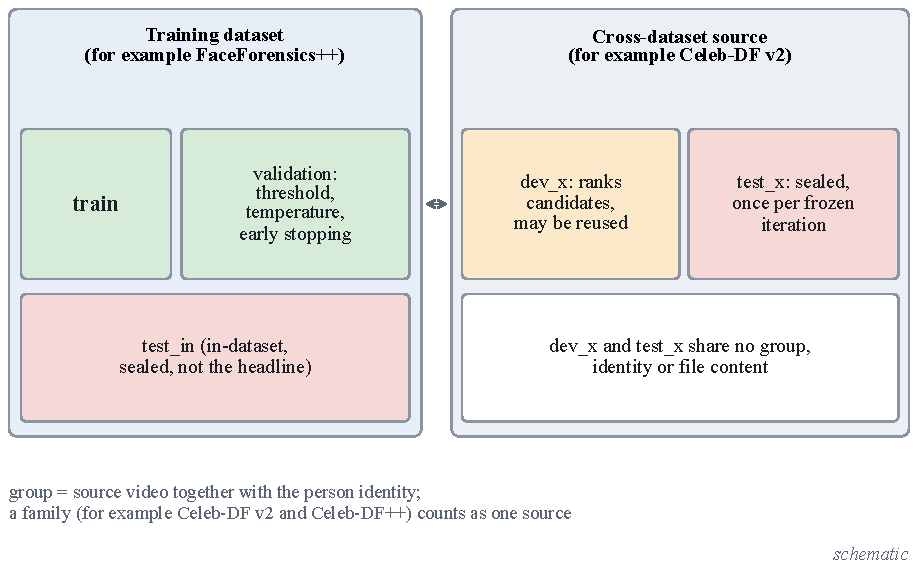
\includegraphics[width=0.96\columnwidth]{fig02_splits.pdf}
\caption[Group-disjoint splits]{Schematic of the splits and of the sealed
reading. The development slice and the sealed tests share no group, identity or
file content with each other or with the training data.}
\label{fig:splits}
\end{figure}

\subsection{Sealed tests, metrics and statistics}
The development slice ranks candidates and judges iterations; it may be read
repeatedly and every verdict on it is exploratory. The sealed sets (\spl{test\_in},
\spl{test\_x}) are read once per frozen iteration through a guarded command that
refuses a sealed split unless the run is flagged final, writes a ledger entry with
the score-file hash, and refuses a second reading without a logged reason; the
final reading produced 74 ledger entries and no repeat. % E-014
The metric is the ROC-AUC, $\mathrm{AUC}=P(S_1>S_0)+\tfrac12P(S_1=S_0)$ for the
scores of a random fake and a random real sample; it uses only ranks and does not
depend on the threshold or the class balance. We also report the equal error rate
(EER), balanced accuracy at the validation threshold and the expected calibration
error with 15 equal-width bins, $\mathrm{ECE}=\sum_b \frac{n_b}{n}|\mathrm{acc}_b-\mathrm{conf}_b|$.
Intervals
are 95\,\% percentile intervals from 2\,000 bootstrap resamples whose unit is the
group, never the clip or frame; with several seeds the metric is averaged over
seeds within each resample. Comparisons are paired on the same resampled groups; post-freeze proportions use
Wilson intervals. Fine-tuning used one seed per learning rate and only base-size
encoders, so that a run fits in 10\,GiB of the 12\,GB card.

\subsection{Confirmatory tests}
Only three tests are confirmatory, declared and committed before the first sealed
read: T1, final minus I-0 on the sealed Celeb-DF family (video); T2, the same on
sealed In-the-Wild (speech); T3, final video system minus a re-run Xception
baseline on the Celeb-DF family. T1 and T2 read ``improved'' if the lower bound of
the paired 95\,\% interval is above zero. For T3, with $L$ that lower bound, non-inferiority is
\begin{equation}
L>-\delta,\qquad \delta=0.0100,
\end{equation}
where $\delta$ was set before the sealed read as twice the larger seed standard
deviation of the baseline with a floor of 0.01; the floor decides. The declared
superiority rule, $L>0$ at the 95\,\% level, is a stricter claim than non-inferiority
and is read together with the Bonferroni line below. Each test also
prints a 98.33\,\% line (Bonferroni over three, same bootstrap draws). It was
declared as a robustness check beside the 95\,\% decision rule; Bonferroni control
holds under any dependence between the three tests, so a reader who wants
family-wise control should read the 98.33\,\% column. Everything else, including
every other sealed number, is exploratory. % D-061, D-062, D-066, D-091

%%%%%%%%%%%%%%%%%%%%%%%%%%%%%%%%%%%%%%%%%%%%%%%%%%%%%%%%%%%%
\section{Results}\label{sec:results}

\subsection{From the working version to the frozen system (exploratory)}
Table~\ref{tab:ladder} follows each change from the limitation that triggered it
to its measured result on the development slice (three seeds), and
Fig.~\ref{fig:ladderres} plots the same values. A change enters only if its
written success line is met. % E-005 to E-013b, E-016, E-017

\begin{table*}[!t]
\centering
\caption[Development ladder]{Development ladder (exploratory; development slice,
mean of three seeds, 95\,\% group-bootstrap interval). Face video: Celeb-DF v2,
15 identities; speech: In-the-Wild, 12 speakers.}
\label{tab:ladder}
\footnotesize
\setlength{\tabcolsep}{3pt}
\begin{tabular}{@{}L{1.7cm} L{4.4cm} L{7.2cm} L{4.0cm}@{}}
\toprule
Step & Limitation and change & Result & Reading \\
\midrule
I-1 video & training AUC 0.8367, frozen feature underfits; full fine-tuning of SigLIP base at $10^{-5}$ &
frozen probe of the same encoder 0.7396 [0.7031, 0.7832], fine-tuned 0.9096 [0.8776, 0.9388]; paired +0.1700 [+0.1228, +0.2114] &
supported; higher rates collapsed \\
Baseline & published family under the same protocol; Xception fine-tuned, same recipe &
0.8716 [0.8364, 0.9076]; SigLIP minus Xception +0.0380 [+0.0172, +0.0592] &
basis of T3 and of $\delta$ \\
I-1b, I-1c video & validation-to-development gap; augmentation with mixup (I-1b), mean of three fine-tuned encoders (I-1c) &
I-1b +0.0219 [+0.0090, +0.0382] on development, $-0.0194$ [$-0.0251$, $-0.0129$] on validation; I-1c +0.0096 [$-0.0020$, +0.0231] &
neither enters: I-1b is a trade-off beyond the allowance 0.0079, I-1c shows no gain \\
\midrule
I-2 speech & recording cues reverse sign; trim silence, peak-normalise &
0.6723 [0.6126, 0.7584]; +0.0623 [+0.0114, +0.1048] &
supported; RMS level cue remains (AUC 0.135 [0.054, 0.382]) \\
I-3 speech & errors on short or saturated clips; noise, low-pass, reverberation, MP3 copies &
0.7455 [0.7052, 0.8121]; +0.0732 [+0.0122, +0.1225] &
supported; 12 speakers \\
I-4 speech & single encoder; mean logit of HuBERT, WavLM, Whisper &
0.8130 [0.7523, 0.8808]; +0.0675 [+0.0300, +0.0929] &
supported; three encoder passes per clip \\
\midrule
I-5, I-6 audio-visual & need audio-visual evidence; frozen heads, then heads trained on LAV-DF with logistic fusion &
frozen: visual 0.3838 [0.3599, 0.4079], audio 0.6476 [0.6244, 0.6701]; trained: fused 0.9935 [0.9905, 0.9962], but visual within produced videos 0.5070 [0.4771, 0.5361] (post hoc control) &
shortcut; no audio-visual detection claim \\
I-7 pulse & rPPG as candidate cue; signal check on 432 real clips against a shuffled control &
0.301 [0.260, 0.346] above control, 0.6 required &
fails; no pulse ground truth \\
\bottomrule
\end{tabular}
\end{table*}

\begin{figure*}[!t]
\centering
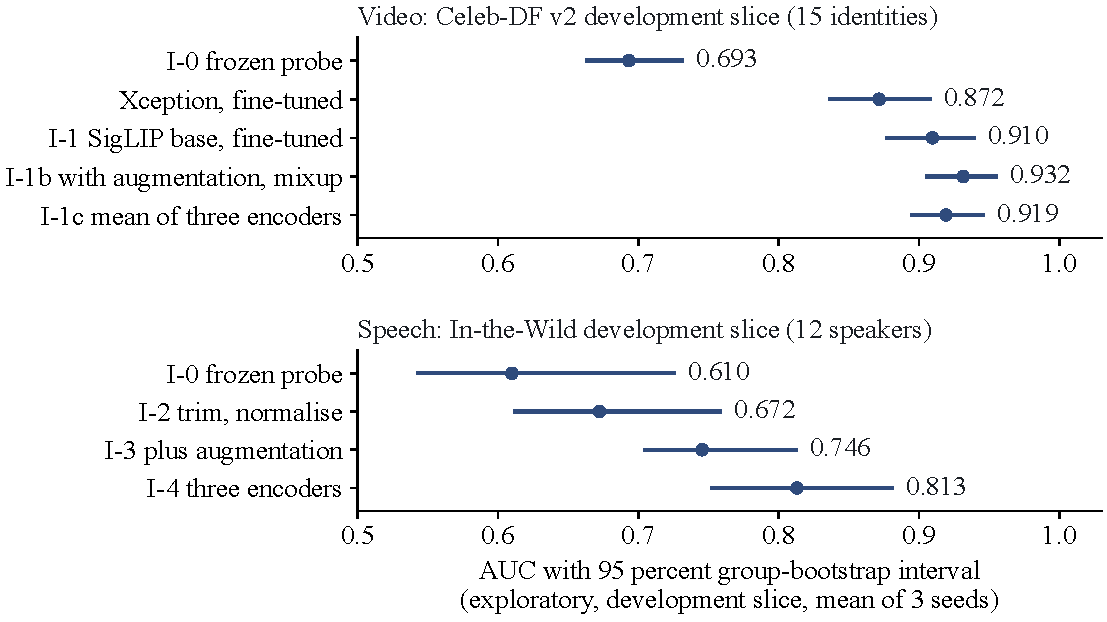
\includegraphics[width=0.74\textwidth]{fig08_ladder_results.pdf}
\caption[Development AUC along the ladder]{Development-slice AUC with the 95\,\%
group-bootstrap interval along the ladder (exploratory, mean of three seeds). The
widths follow from 15 identities (video) and 12 speakers (speech).}
\label{fig:ladderres}
\end{figure*}

\paragraph*{Video}
The gain over the frozen probe of the same encoder (+0.1700 [+0.1228, +0.2114],
15 identities) isolates fine-tuning; the Xception gain over the working version
(+0.1783) is consistent with it but changes the encoder as well. The written
prediction of a gain of at most +0.03 was too small. Two further levers were run on
request although their triggers were not met to the letter, and neither entered.

\paragraph*{Speech}
Each of the three speech changes met its success line, and together they raised
the development AUC from 0.6100 to 0.8130; the point estimates rise and adjacent
intervals overlap. The sealed staircase repeats this (Table~\ref{tab:sealed}). The
first lever, which removes leading silence and level cues, accounts for 0.061 of
the sealed 0.163 gain (0.7516 to 0.8125). % E-007 to E-009, E-014

\paragraph*{Audio-visual and pulse}
The face-video head is below chance on LAV-DF, so fusion was not tested with it.
With heads trained on LAV-DF the fused score reached 0.9935, but a control run
afterwards showed that the visual head separates the data set's produced videos
from its originals, including audio-only fakes whose frames are untouched, and is
at chance within the produced videos (0.5070); a visual head trained on produced
videos only was no better. The audio head is the only one with evidence above chance
inside produced videos (0.8574 on validation). The pulse check found no
recoverable signal; a positive control recovered an injected 1.2\,Hz sinusoid of
relative green amplitude 0.008 in 0.873 of the clips, which shows the pipeline's
sensitivity, not that a pulse exists in compressed video (Fig.~\ref{fig:lavdf}). % E-010 to E-012, E-006, M-005

\begin{figure}[!t]
\centering
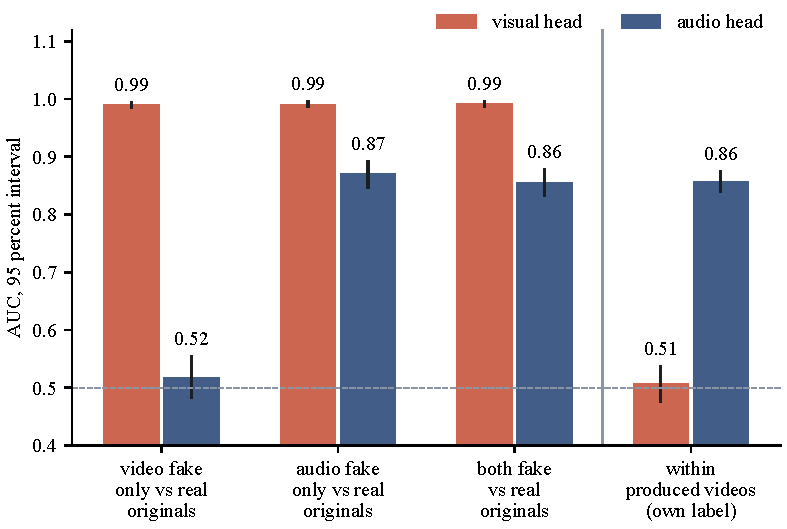
\includegraphics[width=0.96\columnwidth]{fig09_lavdf_cells.pdf}
\caption[LAV-DF per-cell AUC and control]{LAV-DF validation, heads trained on
LAV-DF (exploratory): AUC of each head per kind of fake against the real
originals, and within the produced videos only (control run afterwards).}
\label{fig:lavdf}
\end{figure}

\subsection{Sealed results and confirmatory tests}
The final system (fine-tuned SigLIP for video, the frozen CLIP probe for images,
the three-encoder speech average) was frozen and read once on the sealed sets with
seeds 0 to 2. Table~\ref{tab:sealed} gives the AUCs and Table~\ref{tab:tests} the
three tests. % E-014

\begin{table*}[!t]
\centering
\caption[Sealed-test AUC]{Sealed-test AUC [95\,\% group-bootstrap interval], seeds
0 to 2. Only the Celeb-DF family and In-the-Wild rows feed a confirmatory test;
every other row is sealed but exploratory.}
\label{tab:sealed}
\footnotesize
\setlength{\tabcolsep}{3pt}
\begin{tabular}{@{}L{3.9cm} L{2.0cm} L{2.75cm} L{2.75cm} L{2.75cm} L{1.5cm}@{}}
\toprule
Sealed set & Items / groups & I-0 & Final system & Xception & Role \\
\midrule
Celeb-DF family & 7\,650 / 344 & 0.6238 \ci{0.6015}{0.6486} & 0.8218 \ci{0.8020}{0.8393} & 0.8042 \ci{0.7841}{0.8223} & T1, T3 \\
\quad Celeb-DF v2 test part & 4\,801 / 344 & 0.6322 \ci{0.6018}{0.6658} & 0.8999 \ci{0.8759}{0.9210} & 0.8527 \ci{0.8237}{0.8777} & exploratory \\
\quad Celeb-DF++ fakes, v2 reals & 3\,593 / 344 & 0.6119 \ci{0.5821}{0.6427} & 0.7105 \ci{0.6877}{0.7331} & 0.7351 \ci{0.7083}{0.7599} & exploratory \\
DFD & 3\,431 / 28 & 0.5927 \ci{0.5629}{0.6258} & 0.8797 \ci{0.8566}{0.9041} & 0.8847 \ci{0.8655}{0.9052} & exploratory \\
FaceForensics++ c23 (in-dataset) & 700 / 70 & 0.7946 \ci{0.7667}{0.8243} & 0.9899 \ci{0.9826}{0.9959} & 0.9895 \ci{0.9823}{0.9952} & exploratory \\
\midrule
In-the-Wild & 24\,788 / 42 & 0.7516 \ci{0.6802}{0.8035} & 0.9148 \ci{0.8896}{0.9383} & n/a & T2 \\
\quad after I-2 / I-3 & & & 0.8125 / 0.8672 & n/a & exploratory \\
ASVspoof 2019 LA evaluation (in-dataset) & 71\,237 / 67 & 0.9684 \ci{0.9564}{0.9777} & 0.9835 \ci{0.9798}{0.9872} & n/a & exploratory \\
\midrule
Image: CNN-synthesis & 48\,805 / 16 & 0.9316 \ci{0.8933}{0.9694} & same head & n/a & exploratory \\
Image: diffusion & 10\,000 / 10 & 0.9354 \ci{0.8967}{0.9665} & same head & n/a & exploratory \\
\bottomrule
\end{tabular}
\end{table*}

\begin{table}[!t]
\centering
\caption[Confirmatory tests]{The three confirmatory tests: paired AUC difference
with the declared 95\,\% interval and the 98.33\,\% (Bonferroni over three)
interval.}
\label{tab:tests}
\scriptsize
\setlength{\tabcolsep}{2pt}
\begin{tabular}{@{}L{1.45cm} L{2.2cm} L{1.7cm} L{2.65cm}@{}}
\toprule
Test & 95\,\% (declared) & 98.33\,\% & Reading \\
\midrule
T1 video, final minus I-0 & +0.1980 [+0.1688, +0.2242] & [+0.1627, +0.2303] & improved by the declared rule; holds at 98.33\,\% \\
T2 speech, final minus I-0 & +0.1633 [+0.1177, +0.2266] & [+0.1085, +0.2481] & improved by the declared rule; holds at 98.33\,\% \\
T3 video, final minus Xception & +0.0176 [+0.0025, +0.0327] & [$-0.0011$, +0.0355] & non-inferior at both levels ($\delta=0.0100$); 95\,\% superiority rule met, not after Bonferroni; baseline at 224 px \\
\bottomrule
\end{tabular}
\end{table}

T1 and T2 show that the changes made on the development slices carried over to
sealed data never used for any choice. T3 supports exactly this wording and
nothing beyond it: the final video system is non-inferior to the re-run Xception
at both levels (margin 0.0100); the declared 95\,\% superiority rule was met
but does not survive the Bonferroni correction (98.33\,\% interval [$-0.0011$,
+0.0355]); the baseline ran at 224 pixels and is one network family. On the newer
Celeb-DF++ generators and on DFD, Xception is higher by point estimate. Part of the
0.163 speech gain is the removal of a silence and level shortcut diagnosed on
development data (trimming and normalisation account for 0.061; a level cue
remains, single-feature RMS AUC 0.135 [0.054, 0.382] on the 12-speaker development
slice), so the gain is not all better detection of synthesis. In the training
corpus the leading-silence cue has AUC 0.375 on ASVspoof development data against
0.719 on the In-the-Wild development slice, consistent with a sign-flipped
shortcut; 12 speakers do not establish it. Sealed video values are below the
development values and sealed speech values above them; these are different data
and not a before-and-after pair. On the sealed LAV-DF subset the pattern repeats:
the visual head trained on LAV-DF scores 0.9921 against the fused label but is at
chance within the produced videos (0.5032), where the audio head reaches 0.8480
(exploratory). % E-014; M-004

\subsection{Thresholds and false alarms (post hoc)}
AUC ignores the threshold, but a user sees a threshold decision. Re-analysing
sealed scores already in the ledger, post hoc and not confirmatory, the frozen
video threshold flags 0.1098 of the 744 real videos of the Celeb-DF family and
0.1405 of the 363 real DFD videos, so its false alarms differ between test sets; the
final speech threshold flags 0.1716 of real In-the-Wild clips. The speech equal
error rate is 6.94\,\% [5.94, 7.79] on ASVspoof 2019 LA and 15.78\,\% [12.75,
18.70] on In-the-Wild. % E-032, E-030

\subsection{After the freeze}
Further tests were registered with hypotheses and run without changing the frozen
detectors; the technical report gives them in full. On the sealed identity half of
FakeAVCeleb (5\,013 clips) the pre-stated criteria were met (visual 0.9552
[0.9442, 0.9657], audio 0.9263 [0.9149, 0.9366]), but they are not evidence of
detection quality: the video codec coincides with the manipulation method (codec
metadata alone separates real from fake video at 0.9985 on the development half),
real and fake audio come from different recording channels, and at the frozen
thresholds about half of the fake videos are missed (sensitivity 0.480); thresholds
do not transfer. The image probe reached a macro AUC of 0.7039 [0.6855, 0.7229] on
21 recent generators and missed 0.7395 [0.7300, 0.7500] of their images at its
threshold, part of its separation following the file format. A generated-video head
was at chance on DF26 without DF26 training (0.4957 [0.4755, 0.5168]) and flags most
real clips from other sources, so it detects a video source rather than
generation; a retrained image head ranks better (macro AUC 0.8839, +0.1800
[+0.1643, +0.1959]) but flags 0.5213 of real evaluation images. These experimental
heads give no finding (Table~\ref{tab:post}). % E-015, E-021, E-023, E-019, E-027 to E-029

\begin{table*}[!t]
\centering
\caption[Steps after the freeze]{Steps after the freeze; none changed a frozen
detector. Labels: sealed-exploratory (a held-out or sealed set read once, not
confirmatory) and exploratory (development data).}
\label{tab:post}
\footnotesize
\setlength{\tabcolsep}{3pt}
\begin{tabular}{@{}L{3.3cm} L{8.9cm} L{5.0cm}@{}}
\toprule
Step & Result & Reading \\
\midrule
FakeAVCeleb sealed half (sealed-exploratory) &
visual 0.9552 [0.9442, 0.9657], audio 0.9263 [0.9149, 0.9366]; visual sensitivity 0.480 at specificity 0.996; audio specificity 0.637 &
criteria met, not evidence of detection quality; thresholds do not transfer \\
Codec audit, development half (exploratory) &
metadata alone 0.9985; frozen visual 0.9732 before and 0.8772 after a common re-encode (1\,000-clip sample, not comparable with the sealed value); codec-matched 0.8856 against 0.8763 (+0.0092 [+0.0006, +0.0180]) &
codec explains part, not all; fully confounded with method \\
Generated-video head, DeepAction (DF26 held out once) &
DeepAction 0.8281 [0.7908, 0.8662]; DF26 0.4957 [0.4755, 0.5168], closed generators 0.4880 [0.4534, 0.5204] &
at chance on DF26; experimental only \\
Source-confound test (exploratory) &
338 of 440 unmodified real clips of FaceForensics++ and LAV-DF flagged, 0.7682 [0.7265, 0.8052], against 0.19 of DeepAction reals &
the head separates one library from the rest \\
Head trained on DF26 open generators (exploratory; closed look sealed-exploratory) &
open generators, family left out 0.7453 [0.7174, 0.7710]; closed commercial generators 0.7548 [0.7189, 0.7885] (one counted look; the installed head was at chance there; different real sets); 0.8023 [0.7625, 0.8368] of the 440 real clips flagged &
ranking higher, confound persists: not installed \\
Modern images (sealed-exploratory) &
macro AUC 0.7039 [0.6855, 0.7229] on 11\,550 images; pooled miss rate 0.7395 [0.7300, 0.7500], false alarms 0.0418 [0.0368, 0.0470]; format-only macro AUC 0.9301 &
inadequate by the line fixed in advance; format confounded with label \\
Portrait check (sealed-exploratory) &
3\,119 face images: whole-image AUC 0.7859 [0.7717, 0.7995], miss rate 0.8063; face path 0.6020; paired +0.1839 [+0.1596, +0.2074] &
better than the face path, not usable \\
Retrained image head (sealed-exploratory) &
macro AUC 0.8839 [0.8732, 0.8942]; +0.1800 [+0.1643, +0.1959] over the installed head; false-alarm rate 0.5213 [0.5091, 0.5339] &
ranking supported; not eligible \\
Lip-sync check (exploratory) &
false alarms 1.3\,\% [0.4, 3.8] (old rule 11.7\,\%) on 230 held-out real clips; Wav2Lip flagged 0 of 160 &
weak evidence, not a detector \\
\bottomrule
\end{tabular}
\end{table*}

\paragraph*{Why the experimental heads were not accepted}
A detector enters the product only through an approval table, and the table is
empty. The generated-video heads rank their own benchmark but flag most unmodified
real clips from other sources (0.7682 and 0.8023 of 440), so they detect a video
source, not generation. The retrained image head fails the eligibility line fixed
in advance (AUC lower bound at least 0.85, false-alarm upper bound at most 0.10,
JPEG drop below 0.10): its false-alarm rate is 0.5213, and re-fitting its
threshold on the evaluation images would be test tuning, so it was not done. The
whole-image portrait check beats the face path on the same images but misses 0.8063
of generated faces. % D-074, D-083, D-085, D-086; E-025

\paragraph*{Gemini-generated images}
No Gemini data was downloaded, no model trained and nothing evaluated; the system
has no Gemini capability. The nearest measured proxy is Google Imagen~3, one of
the 21 generators above: the frozen head reached AUC 0.7691 [0.7352, 0.8020] and
missed 0.8719 of its images, and a PNG-only format score separates the cell at
0.9731, so it is confounded by file format. Imagen~3 is not Gemini. The provider's
terms for using outputs to train a detector, provenance, matched real controls and
model-version coverage are unresolved, so a registered Gemini study is
blocked. % GEMINI_FEASIBILITY; E-028, E-029

\subsection{Comparison with published results}\label{sec:compare}
A published number receives a computed difference only when task, data, protocol
and metric match. The only such row is our re-run Xception baseline (T3). Our
speech EER on ASVspoof 2019 LA (6.94\,\% [5.94, 7.79]) is given next to the 1.13\,\%
that the AASIST authors quote~\cite{jung2021aasist}; AASIST was not re-run, so this
is context, and whether it transfers better was not measured on a common protocol.
DeepfakeBench reports a frame-level Xception AUC of 0.7365 on Celeb-DF
v2~\cite{yan2023deepfakebench}, against our video-level values on a different
test subset; no ordering is drawn. On a different test set, with no ranking, the full In-the-Wild set gives 33.9\,\% in~\cite{muller2022inthewild} and 7.2\,\% in~\cite{pascu2024generalisable}, against our
15.78\,\% on 42 of its speakers. On DF26 our head is at chance without DF26 training
(0.4957 [0.4755, 0.5168]); the DF26 authors report 44.0 to 69.7 for
FaceForensics++-trained detectors without intervals~\cite{shykula2026df26}; training
data and frame sampling differ, so no ordering is drawn.

%%%%%%%%%%%%%%%%%%%%%%%%%%%%%%%%%%%%%%%%%%%%%%%%%%%%%%%%%%%%
\section{Discussion}\label{sec:disc}
On the protocol fixed in advance, the changes made on small development slices
carried over to sealed data: fine-tuning for face video and three preprocessing
and ensembling steps for speech improved on the first version by the declared rule
(T1, T2), with the speech caveat above, and against a re-run published network
family the video system is non-inferior at both levels. The same evidence shows
where the system stops. Scores order clips from sources unlike the training data
better than the first version's did, but thresholds fixed on validation data do
not transfer, so a flag carries high uncertainty and a score is a ranking, not a
probability. That is why the platform of the technical report gives cautious
per-module findings and never one number per file.

%%%%%%%%%%%%%%%%%%%%%%%%%%%%%%%%%%%%%%%%%%%%%%%%%%%%%%%%%%%%
\section{Limitations}\label{sec:discussion}
\begin{itemize}
  \item \emph{Small slices and groups.} Development slices hold 15 identities, 12
        speakers and 2 generator units, so every iteration verdict is exploratory
        and intervals are wide. Sealed video rests on 344 groups, strongly
        imbalanced (744 real against 6\,906 fake) and mixing two sources; sealed
        speech on 42 speakers.
  \item \emph{One sealed run, one baseline.} Each frozen iteration was read once; T3
        uses one baseline family at 224 px, $\delta$ sits at its floor, the
        baseline's learning rate lies at the edge of its grid, and T3 does not hold
        at the Bonferroni level.
  \item \emph{Speech shortcut.} Part of the speech gain removes a silence and level
        shortcut; a level cue remains, and 42 speakers are few.
  \item \emph{Thresholds and false alarms.} Thresholds fixed on validation data do
        not transfer: the video threshold misses about half of the FakeAVCeleb fakes
        and flags 0.1098 and 0.1405 of the real videos of the Celeb-DF family and
        DFD (post hoc), and scores are not probabilities on other sources.
  \item \emph{Dataset artefacts.} Codec (FakeAVCeleb), file format and size
        (Community Forensics) and a production cue (LAV-DF) inflate AUC; controls
        reduce but do not remove them. No audio-visual detection, pulse signal or
        generated-video detection is claimed.
  \item \emph{Records and licences.} Some post-freeze registrations entered version
        control together with their scripts, so their order rests on the project's
        own record. All data are research-only; the OpenAI CLIP and WavLM weights
        are used as research-only and the SyncNet weights state no licence.
\end{itemize}

%%%%%%%%%%%%%%%%%%%%%%%%%%%%%%%%%%%%%%%%%%%%%%%%%%%%%%%%%%%%
\section{Conclusion}\label{sec:concl}
We built a local multimodal checker and recorded every step that shaped it. A
simple first version with frozen encoders showed where it failed; fine-tuning the
video encoder and three speech changes addressed the measured weaknesses on
development data, and on sealed data the frozen system improved on the first
version by the declared rule (video +0.1980, speech +0.1633). It is non-inferior
to a re-run Xception at both levels, while its 95\,\% superiority does not survive
the Bonferroni correction. Audio-visual fusion, pulse signals, generated-video
heads and a retrained image head were tested and not accepted, each for a measured
reason, and the frozen thresholds do not transfer. Future work, as recorded in the
project plan: scoring the frozen face system on the official Celeb-DF v2 test list
beside the baseline, adapting a larger encoder~\cite{hu2022lora}, a threshold
calibrated on diverse real sources, and the Gemini study once its blockers are
resolved.

%%%%%%%%%%%%%%%%%%%%%%%%%%%%%%%%%%%%%%%%%%%%%%%%%%%%%%%%%%%%
\bibliographystyle{IEEEtran_hyphen}
\bibliography{refs}

\end{document}
